\subsection{Obiettivi del prodotto}
	L'obiettivo del prodotto è quello di fornire agli utenti una piattaforma online in cui sia possibile trovare, creare e svolgere esercizi di analisi grammaticale, con lo scopo di poter formare un correttore automatico raccogliendo e immagazzinando i dati. 
La proponente ha imposto i seguenti vincoli sull'implementazione del prodotto:

\subsubsection{Obbligatori}
\begin{itemize}
	\item l'utente deve poter chiedere al sistema di svolgere automaticamente un esercizio mediante un software basato sull'apprendimento supervisionato;
	\item l'utente deve poter correggere l'output automatico generato dal correttore e di salvare il risultato finale;
	\item l'utente deve poter scaricare i dati collezionati nella piattaforma.
\end{itemize}
\subsubsection{Desiderabili}
\begin{itemize}
	\item l'utente dovrebbe avere la possibilità di svolgere e correggere gli esercizi in più lingue;
	\item l'utente dovrebbe avere la possibilità di personalizzare i dati prima di scaricarli dalla piattaforma;
	\item l'utente dovrebbe avere la possibilità di differenziare tra dati pubblici e privati.
\end{itemize}
\subsubsection{Opzionali}
\begin{itemize}
	\item l'utente potrebbe voler salvare l'intera cronologia delle modifiche di alcuni dati;
	\item l'utente potrebbe voler creare e/o scaricare un modello direttamente dalla piattaforma.
\end{itemize}

\subsection{Tipologie di utenti}
Gli utenti sono suddivisibili in tre principali categorie: 
\begin{itemize}
	\item \textbf{Moderatore:} si occupa di verificare che le persone rispettino il codice di comportamento della piattaforma e della gestione degli esercizi presenti in essa;
	\item \textbf{Sviluppatore:} è interessato alla consultazione dei dati raccolti, magari applicando filtri o visualizzando lo storico delle annotazioni;
	\item \textbf{Utente generico:} è la tipologia di utente più comune che è interessato alla ricerca e allo svolgimento di esercizi sulla piattaforma.
\end{itemize}

Quest'ultima categoria è suddivisibile ulteriormente in:
\begin{itemize}
	\item \textbf{Utente non riconosciuto:} è l'utente che non ha il pieno accesso alle funzionalità dell'applicazione.
	\item \textbf{Utente riconosciuto:} è l'utente che ha le credenziali e ha effettuato l'accesso.
\end{itemize}

L'utente riconosciuto individua due sottocategorie:
\begin{itemize}
	\item \textbf{Allievo:} gli allievi possono iscriversi alle classi, gestire tali iscrizioni e visualizzarne i dati. // RIVEDERE
	\item \textbf{Insegnante:} gli insegnanti possono inserire soluzioni degli esercizi, gestire le proprie classi e visualizzare il rendimento dei propri alunni.
\end{itemize}
\begin{figure}[h]
			\centering
			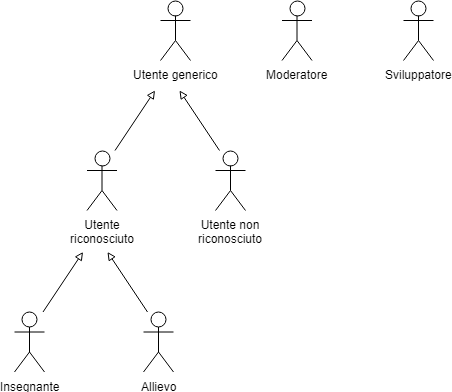
\includegraphics[scale=0.7]{images/attori.png}
			\caption{Attori del progetto}
		\end{figure}